\chapter{Panoramica del progetto}
\begin{minipage}{12cm}\textit{Nel capitolo verr\`{a} effettuata una breve introduzione alle componenti principali del progetto, verr\`{a} esposto il percorso di progettazione seguito per un suo corretto sviluppo, e illustrato l'utilizzo del software da parte dell'utente.}
\end{minipage}

\vspace*{1cm}
\section{Componenti principali}
Le entit\`{a} principali presenti nel software realizzato sono un \textit{Parser}, con il ruolo di interpretare le informazioni contenute nel file di configurazione, uno \textit{Scheduler}, che ha il compito di garantire la corretta esecuzione dei task al termine delle rispettive scadenze, un protocollo di comunicazione (\textit{HTTP}) con cui interrogare le macchine specificate. Nello sviluppo dell'applicativo \textit{multi-piattaforma} \`{e} stato utilizzato il \textit{Singleton pattern}, per evitare la creazione di istanze multiple dello scheduler o del logger.
In ottica di una futura integrazione del software in una rete di bot, sono state inserite funzioni per il calcolo di un ID univoco per ogni macchina appartenente alla rete controllata.

\vspace*{0.5cm}
\subsection{HTTP}
\textbf{HTTP}, acronimo di \textit{hypertext transfer protocol}.
\`E un protocollo a livello applicativo utilizzato per la
trasmissione di informazioni tramite un meccanismo di richiesta/risposta tra \textit{client} e \textit{server}. All'interno del messaggio di richiesta sono definiti diversi campi tra cui il tipo di
richiesta (\textit{GET}, \textit{POST}) e lo \textit{UserAgent}, che identifica la tipologia di \textit{client} utilizzata.
Il metodo \textit{GET} pu\`{o} essere utilizzato per effettuare una richiesta:
\begin{itemize}
	\item \textbf{assoluta}, senza ulteriori specificazioni sulla risorsa cercata;
	\item \textbf{condizionale}, se nell'\textit{header} del messaggio di richiesta sono presenti i campi \textit{If-Modified-Since}, \textit{If-Match}, etc.;
	\item \textbf{parziale}, quando la risorsa richiesta \`e una sottoparte di una risorsa memorizzata.
\end{itemize}
Nel software sono effettuate solo \textit{GET} assolute, e la scelta dello \textit{user-agent} \`{e} lasciata alla discrezione dell'utilizatore.

\vspace*{0.5cm}
\subsection{Singleton Pattern}
In determinati contesti \`e necessario che venga istanziato un solo esemplare di una classe. Ad esempio: per evitare due riproduzioni audio contemporanee, sar\`{a} opportuno istanziare un riproduttore musicale una sola volta,
uno \textit{spooler} di stampa dovrebbe tenere una coda unica anche se sono presenti pi\`{u} stampanti attive e
il manager di un file system dovrebbe essere unico.

Per garantire questa singola istanziazione \`{e} sufficiente rendere impossible l'utilizzo del costruttore della classe da parte del resto del codice, e fornire un metodo indiretto per ottenere una istanza (l'unica) di tale classe.
Sono quindi possibili diverse soluzioni:
\begin{itemize}
	\item dichiarare privato il costruttore, in modo che esso possa essere visto solo all'interno della classe Singleton;
	\item prevedere il metodo (pubblico) statico e cio\`e di classe, in modo che esso sia comunque visibile. Questo metodo deve istanziare un esemplare se ci\`o non \`e ancora accaduto, oppure restituire l'oggetto gi\'a istanziato in precedenza senza istanziare ulteriori esemplari.
\end{itemize}
Questa seconda scelta \`e quella applicata nel progetto per la creazione e gestione del \textit{logger} e la creazione di uno schedulatore di task.

\vspace*{0.5cm}
\subsection{Scheduler}
Lo \textit{scheduler} ha il compito di garantire la corretta esecuzione dei task al termine delle rispettive scadenze.

Nell'applicativo \`{e} stato utilizzato uno \textit{Scheduler Executor Service}, istanziato una sola volta mediante l'uso del \textit{Singleton pattern}; data la presenza di istruzioni bloccanti nei task da eseguire, \`{e} stato messo a disposizione dello scheduler un pool di $30$ \textit{thread}.

La classe utilizzata permette la schedulazione di job periodici tramite la funzione \textit{scheduleAtFixedRate} ma, data la necessit\`{a} di schedulare task con rate non fissato, \`{e} stato deciso di effettuare le singole ri-schedulazioni utilizzando, la pi\`{u} semplice, funzione \textit{schedule}.


\vspace*{0.5cm}
\subsection{ID dei bot e MD5}
In una rete reale, i \textit{bot} sono univocamente identificabili dal centro di comando e controllo:
l'attaccante ha interesse nel conoscere il numero di \textit{bot} attivi per effettuare un attacco ad una data; questa informazione inoltre risulta fondamentale, a livello economico, se egli decide di vendere o affittare la \textit{botnet} ad un acquirente esterno. 

Per garantire l'unicit\`{a} dell'identificativo di ogni bot, viene effettuato l'\textit{hash md5} delle informazioni riguardanti l'hardware della macchina e il sistema operativo in esecuzione.

\vspace*{0.5cm}
\subsection{Parsing}
La corretta interpretazione del file di configurazione \`{e} garantita dal \textit{Parser} che, mediante la conoscenza del protocollo utilizzato per l'organizzazione delle informazioni e la manipolazione di oggetti di tipo stringa, genera dal file l'\textit{ArryList} dei task in attesa di esecuzione. 

La classe \`{e} utilizzata anche per l'operazione di scrittura del file di configurazione a partire dai \textit{form} riempiti dall'utente nell'interfaccia principale dell'applicazione.

\vspace*{0.5cm}
\subsection{Multi-piattaforma}
Quando si parla di un programma multi-piattaforma si intende un programma in grado di funzionare correttamente su diversi sistemi operativi.\\
Sono stati gestite quindi le funzionalit\`{a} dipendenti dalla piattaforma su cui l'applicativo \`{e} in esecuzione (come la generazione dell' ID univoco del bot o l'individuazione dei browser installati), differenziandone il comportamento sulla base del sistema operativo presente sulla macchina.

\vspace*{0.5cm}
\section{Piattaforma di sviluppo, Swing, Awt}
NetBeans \`e un ambiente di sviluppo integrato (\textit{IDE} -  \textit{Integrated Development Environment}) multi-linguaggio, scelto dalla Oracle Corporation come \textit{IDE} ufficiale da contrapporre al pi\'u diffuso Eclipse.\\
NetBeans utilizza due componenti principali: la piattaforma, che comprende una serie di librerie per fornire gli elementi base dell'\textit{IDE} come presentazione dei dati e interfaccia utente, e l'\textit{IDE} vero e proprio, che permette di gestire il controllo e le funzionalit\'a offerte dalla piattaforma. NetBeans utilizza \textit{Abstract Window Toolkit} (\textit{AWT}), un insieme di API realizzate da Sun che permettono agli sviluppatori di modellare le interfacce grafiche delle finestre, pulsanti e altri elementi visuali. \textit{AWT} fornisce gli elementi grafici base che dipendono dalla piattaforma utilizzata, mentre per gli aspetti di alto livello come gestione di colori e interazione con l'utente \`e usata la libreria Swing.

\vspace*{1cm}
\section{Build your own botnet}
In questa sezione sono presentati la struttura del progetto ed i principali casi d'uso dell'applicativo realizzato.

\vspace*{0.5cm}
\subsection{Struttura del progetto}
Il progetto \`e composto da diverse classi:
\begin{itemize}
\item \textbf{ByobComm}, responsabile del protocollo di comunicazione;
\item \textbf{ByobSingleton}, tramite il quale \`{e} stato implementato il \textit{Singleton pattern};
\item \textbf{ByobTask}, rappresenta il singolo \textit{task} che deve essere schedulato;
\item \textbf{Byob\_v1}, la classe principale, da cui viene avviata la GUI;
\item \textbf{GUI}, responsabile di ci\`{o} che riguarda la creazione e gestione della \textit{Graphic User Interface} ;
\item \textbf{Parser}, responsabile della creazione di file, lettura e scrittura dei parametri di configurazione inseriti dall'utente;
\item \textbf{Tools}, contenente varie funzioni e metodi utili in diversi contesti;
\item \textbf{URLDetails}, contenente i dati (parametri di configurazione) del singolo \textit{contatto} da effettuare.
\end{itemize} 

\vspace*{0.5cm}
\subsection{ByobComm}
La classe \textit{ByobComm} gestisce la comunicazione HTTP.
Se presente, viene configurato il \textit{proxy} specificato nel file di configurazione; si specifica il tipo di metodo HTTP utilizzato (GET), la codifica dell'\textit{header} e lo \textit{user agent}.
Per la connessione si \`{e} utilizzata la classe \textit{HttpURLConnection}.

\vspace*{0.5cm}
\subsection{ByobSingleton}
Responsabile del \textit{Singleton pattern} utilizzato, contiene al suo interno il \textit{Logger} dell'applicazione, che trascrive:

\begin{itemize}
\item i contatti e i parametri di configurazione;
\item il \textit{timestamp} di contatto e il dettaglio delle URL contattate;
\item le informazioni relative al Sistema Operativo e ai browser presenti sulla postazione su cui il software \`e installato.
\end{itemize}
Oltre al \textit{Logger}, la classe comprende al suo interno lo \textit{scheduler} dei \textit{task} da eseguire.

\vspace*{0.5cm}
\subsection{ByobTask}
\textit{ByobTask} rappresenta il singolo task che lo \textit{Scheduler Executor Service} deve eseguire.
Essa implementa l'interfaccia \textit{Runnable}, ed ogni istanza della classe ri-schedula la propria esecuzione in accordo con le informazioni immagazzinate nel contatto \textit{URLDetails} a cui \`{e} associata.

\vspace*{0.5cm}
\subsection{GUI}

La classe \textit{GUI} rappresenta l'interfaccia grafica tramite la quale l'utilizzatore pu\`{o} fornire i parametri di configurazione dell'applicazione.
Le azioni principali che possono essere intraprese sono due:
\begin{enumerate}
\item l'apertura di un file di configurazione gi\`{a} compilato (\textbf{Figura \ref{fig:gui}});
\item la creazione di un nuovo file di configurazione.
\end{enumerate}

\begin{figure}[!htb]
	\centering
	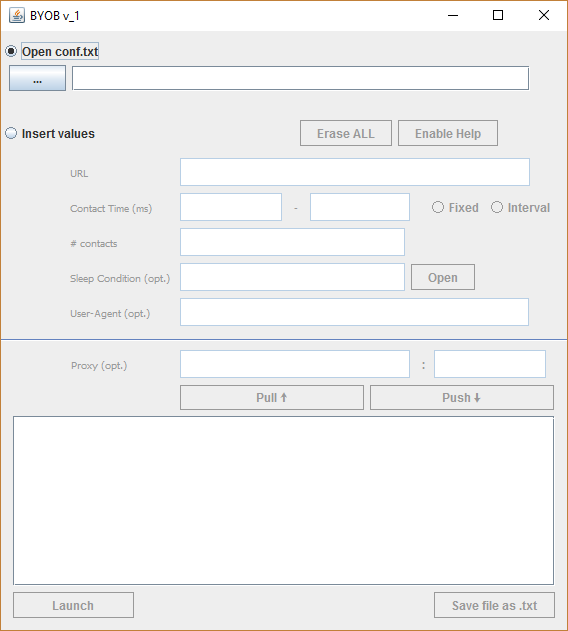
\includegraphics[width=0.7\linewidth]{./imgs/gui}
	\caption{Apertura di un file di configurazione}\label{fig:gui}
	\vspace*{0.5cm}
\end{figure}

\begin{figure}[!htb]
        \centering
		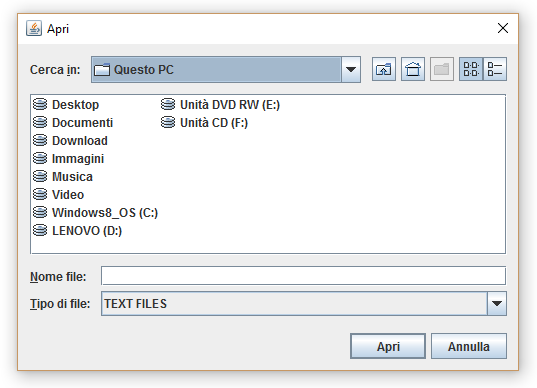
\includegraphics[width=0.6\linewidth]{./imgs/scelta1}
        \caption{JFileChooser}
        \label{fig:chooser}
\end{figure}

Alla pressione del tasto "...", un \textit{JFileChooser} permetter\`{a} la ricerca di un file di testo all'interno delle directory presenti nel dispositivo di memorizzazione in uso (\textbf{Figura \ref{fig:chooser}}).

\begin{figure}[!htb]
        \centering
		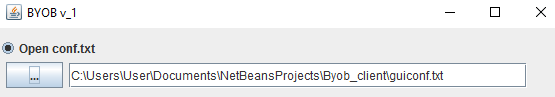
\includegraphics[width=0.7\linewidth]{./imgs/scelta11}
        \caption{Scelta del file di configurazione}
        \label{fig:conf}
\end{figure}

Una volta effettuata la selezione, il percorso assoluto del file scelto verr\`{a} scritto nella casella di testo relativa, e sar\`{a} attivato il tasto "Launch" per l'avvio dell'applicazione (\textbf{Figura \ref{fig:conf}}).

\begin{figure}[!htb]
        \centering        
        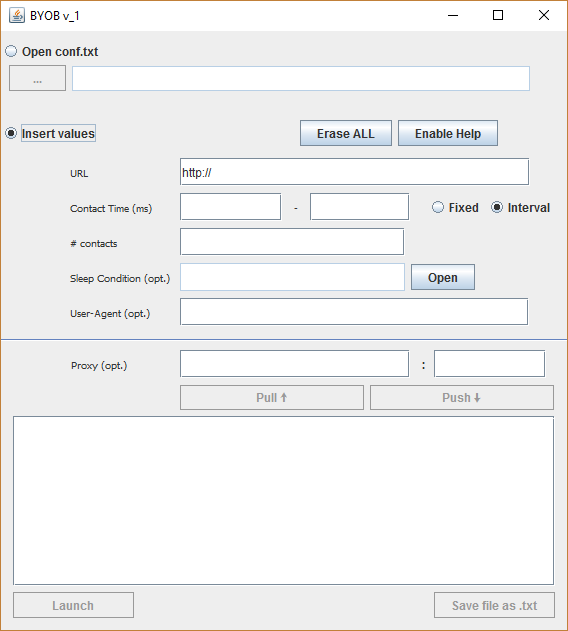
\includegraphics[width=0.7\linewidth]{./imgs/gui2}
        \caption{Inserimento manuale parametri di configurazione}
        \label{fig:manual}
\end{figure}

Tramite l'inserimento manuale dei parametri di configurazione, \`{e} possibile specificare (\textbf{Figura \ref{fig:manual}}):

\begin{itemize} 
\item la \textbf{URL} da contattare;
\item il \textbf{Contact Time}, ossia la periodicit\`{a} di contatto che pu\`{o} essere:
\begin{itemize}
\item [-] Fissa ("\textit{Fixed}");
\item [-] Invervallo ("\textit{Interval}"), cio\`e all'interno di un intervallo temporale;
\end{itemize} 
\item \textbf{\#contacts}, ossia il numero massimo di contatti da effettuare verso la URL specificata;
\item le \textbf{Sleep conditions} (campo opzionale), ovvero l'insieme delle condizioni temporali sotto le quali non deve essere svolta alcuna azione; 
\begin{figure}[!htb]
        \centering
		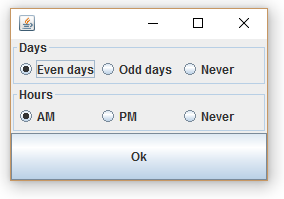
\includegraphics[width=0.4\linewidth]{./imgs/sleep}
        \caption{Sleep conditions}
\end{figure}
\begin{itemize}
\item [-] Condizione sui giorni pari (E), sui giorni dispari (O), nessuna restrizione;
\item [-] Condizione sulle prime dodici ore (A), condizione sulle ultime 12 ore (P), nessuna restrizione;
\end{itemize}
\item lo \textbf{User-Agent} (opzionale), ossia la modifica da apportare al campo User-Agent dell'header HTTP;
\item il \textbf{Proxy} (opzionale), ossia l'indirizzo IP e la porta di un proxy pubblico da utilizzare.
\end{itemize} 

Una volta inseriti nelle relative caselle di testo, il tasto "\textit{Push}" permette di visualizzare tali parametri nell' area sottostante (\textbf{Figura \ref{fig:push}}). 

Il tasto "\textit{Pull}" permette di estrarre dall'area di testo l'ultimo inserimento effettuato per una eventuale modifica dei parametri non correttamente inseriti.
\begin{figure}[!htb]
        \centering
		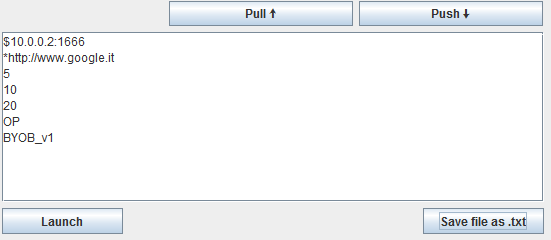
\includegraphics[width=0.6\linewidth]{./imgs/textarea}
        \caption{Push - Inserimento dell'input nell'area di testo}
        \label{fig:push}
        \vspace*{0.5cm}
\end{figure}

Al termine dell'inserimento manuale, la pressione del tasto "Save file as .txt" permette il salvataggio, tramite procedura guidata, del file di configurazione appena creato.

\paragraph{GUI user-friendly}
La pressione del tasto "Enable Help" permette la comparsa (al passaggio del mouse) di \textit{tooltip} sulle caselle del form, rendendone pi\`{u} immediata la corretta compilazione (\textbf{Figura \ref{fig:help}}).

\begin{figure}[!htb]
        \centering        
        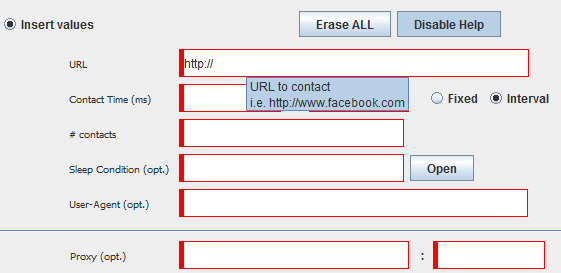
\includegraphics[width=0.7\linewidth]{./imgs/help}
        \caption{Utilizzo dell'help}
        \label{fig:help}
\end{figure}

La pressione del tasto "Erase ALL", da utilizzare in caso di molteplici errori, causa la cancellazione di tutto il file di configurazione compilato.

Nel caso vengano riscontrati degli errori al momento della pressione del tasto "Push", un popup guider\`{a} l'utilizzatore nella risoluzione dei problemi individuati (\textbf{Figura \ref{fig:warning}}).

\begin{figure}[!htb]
        \centering        
        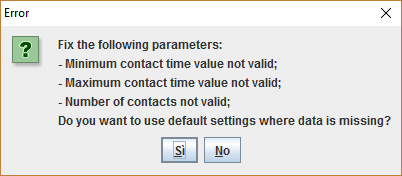
\includegraphics[width=0.6\linewidth]{./imgs/warning}
        \caption{Esempio di messaggio d'errore per dati mancanti e/o errati}
        \label{fig:warning}
\end{figure}

\vspace*{0.5cm}
\subsection{Parser}
La classe \textit{Parser} \`{e} responsabile di:
\begin{itemize}
\item lettura e scrittura del file contenente i parametri di configurazione;
\item creazione di una lista di istanze della classe \textit{URLDetails}, una per ciascun contatto da effettuare;
\item conversione dei parametri di configurazione;
\item controllo di validit\`{a} per ciascun parametro di configurazione.
\end{itemize}

\vspace*{0.5cm}
\subsection{Tools}
La classe \textit{Tools} contiene al suo interno diversi metodi statici, utili in pi\`{u} sezioni del programma.
Essa \`{e} responsabile della generazione dell'ID del bot, della prima schedulazione dei task programmati, della raccolta delle informazioni relative al sistema operativo e ai browser installati sulla macchina, dei controlli per la generazione dei \textit{warning messages} della classe GUI.

\vspace*{0.5cm}
\subsection{URLDetails}
\textit{URLDetails} \`e la classe che contiene le informazioni inserite dall'utente per ciascun contatto che deve essere effettuato.